\documentclass[12pt]{article}

\usepackage[margin=1in]{geometry}
\usepackage{fancyhdr}
\usepackage{amsmath, amsfonts, amsthm, amssymb, mathtools}  % Some math symbols
\usepackage{color}
% \usepackage{sectsty}
\usepackage{tcolorbox}
\usepackage{amsfonts}
\usepackage{titletoc}
\usepackage{caption}
\usepackage[normalem]{ulem}
\usepackage{graphicx}


\usepackage{hyperref}
\hypersetup{
    colorlinks,
    citecolor=black,
    filecolor=black,
    linkcolor=black,
    urlcolor=black
}


\titlecontents{section}[0em]
{\smallskip}
{\thecontentslabel\enspace}
{\hspace*{-5.3em}}
{\hfill\contentspage}



%%%%%%%%%%%% SETUP %%%%%%%%%%%%

% name of the class
\newcommand{\classname}{CSE 371}
% name of the assignment
\newcommand{\assignmentname}{HW3}
% collaborators on assignment
\newcommand{\collaborators}{Cameron Jennings (ID: 2029631), Donovan Clay (ID: 2276005)}
\newcommand{\listcollaborators}{Collaborators: \collaborators}

\pagestyle{fancy}
\fancyhf{}
\setlength{\headheight}{13.59999pt}
\rhead{\thepage}
\lhead{\hyperref[beginning]{\classname \hspace{1em} \assignmentname}}

\usepackage{titlesec}
\titleformat{\subsection}{\normalfont\fontsize{12}{15}\bfseries}{\thesubsection}{1em}{}

\titleformat{\section}[block]
{\filcenter\large
\addtolength{\titlewidth}{2pc}%
\titleline*[c]{}%
\addvspace{6pt}%
}
{\thesection}{1em}{}
\titlespacing{\section}
{5pc}{*2}{*2}[5pc]


% \definecolor{WordSectionBlue}{RGB}{30, 90, 147}
% \allsectionsfont{\color{WordSectionBlue}}

%%%%%%%%%%%% FILE SPECIFIC IMPORTS %%%%%%%%%%%%

\usepackage{ragged2e}
\usepackage{tikz}

%%%%%%%%%%%%%%%%%%%%%%%%%%%%%%%%%%%%%%%%%%%%%%%

\renewcommand*{\thesection}{Question \arabic{section}.}
\renewcommand{\thesubsection}{(\alph{subsection})}

%%%%%%%%%%%% ENVIRONMENTS %%%%%%%%%%%%

\newenvironment{explanation}{\begin{tcolorbox}[colback=blue!2!white,colframe=blue!20!white]}{\end{tcolorbox}}

\newenvironment{subquestion}[1]{\subsection{#1}
\begin{tcolorbox}[colback=blue!2!white,colframe=blue!20!white]}{\end{tcolorbox}}

\newenvironment{sssq}[3]{\textbf{\thesubsubsection.\sssqARG{#1}} \hspace{0.5cm}
\begin{minipage}[t][\sssqARG{#2}][t]{14cm}
    \textbf{\sssqARG{#3}}
\end{minipage}
\begin{explanation}
}{\end{explanation}}

%%%%%%%%%%%% MY MACROS %%%%%%%%%%%%

\newcommand{\prob}{\mathbb{P}}
\newcommand{\expect}{\mathbb{E}}
\newcommand*\sssqARG{}
\newcommand{\bayes}{\textbf{Bayes' Theorem}}
\newcommand{\ltp}{\textbf{Law of Total Probability}}
\newcommand{\var}{\text{Var}}
\newcommand{\unif}{\sim \text{Unif}}
\newcommand{\expo}{\sim \text{Exponential}}
\newcommand{\caseif}{\text{if }}
\newcommand{\nlog}{\text{ln}}


%%%%%%%%%%%%%%%%%%%%%%%%%%%%%%%%%%%%%%
\begin{document}

    \setcounter{tocdepth}{1}
    \begin{center}\label{beginning}
        \tableofcontents 
    \end{center}

    \begin{center}
        \listcollaborators
    \end{center}

    % fix section heading font
    \titleformat{\section}{\normalfont\fontsize{17.28}{15}\bfseries\raggedright}{\thesection}{1em}{}
    \newpage
    \AddToHook{cmd/section/before}{\clearpage}

    % Question 1
    \section{}
        \begin{subquestion}{Breifly explain your approach. Describe a high level the change you made to the code and how you verified that it works correctly.}
            Our approach was to change the lower-level modules first and use testbenches to verify they have the expected behavior. That started with the reg file by changing it so we can write 16 bits at a time. \\
            
            We then changed the controller to accomodate the logic of writing 16 bits at a time. This includes incrementing the write address by two, and changing it so that the buffer is full when the read and write pointers are within 1 address apart. \\

            We ensured the \texttt{reg\_file} module was working by using a testbench to demonstrate that we could write 16 bits with the MSB and LSB in the correct order in the buffer. We then ensured the \texttt{fifo\_ctrl} module was working by using a test bench to demonstrate that reading and writing moves the correct pointers and the \texttt{full} signal was asserted when the buffer was actually full. \\
            
            We then ensured the \texttt{fifo} was working by using a testbench to demonstrate that we could write to the buffer (16 bits at a time) and read from the buffer (8 bits at a time).
        \end{subquestion}

        \begin{subquestion}{Simulation Results}
            Reg File Simulation:
            \begin{center}
                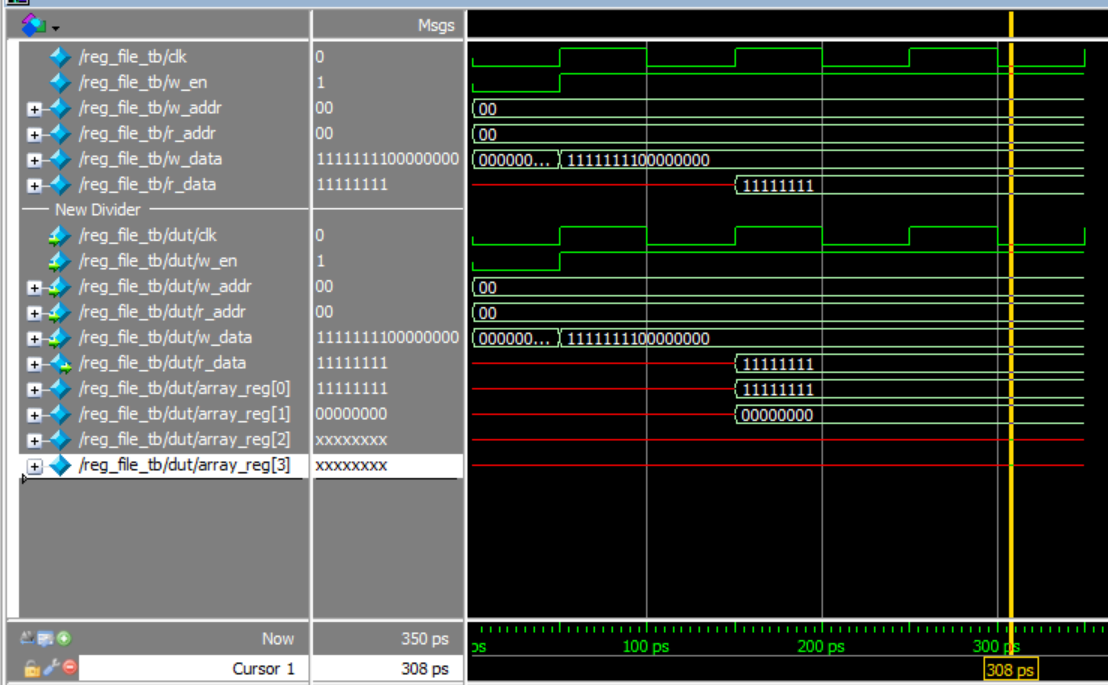
\includegraphics[scale=0.5]{Images/reg file simulation.png}
            \end{center}

            Fifo Ctrl Simulation:
            \begin{center}
                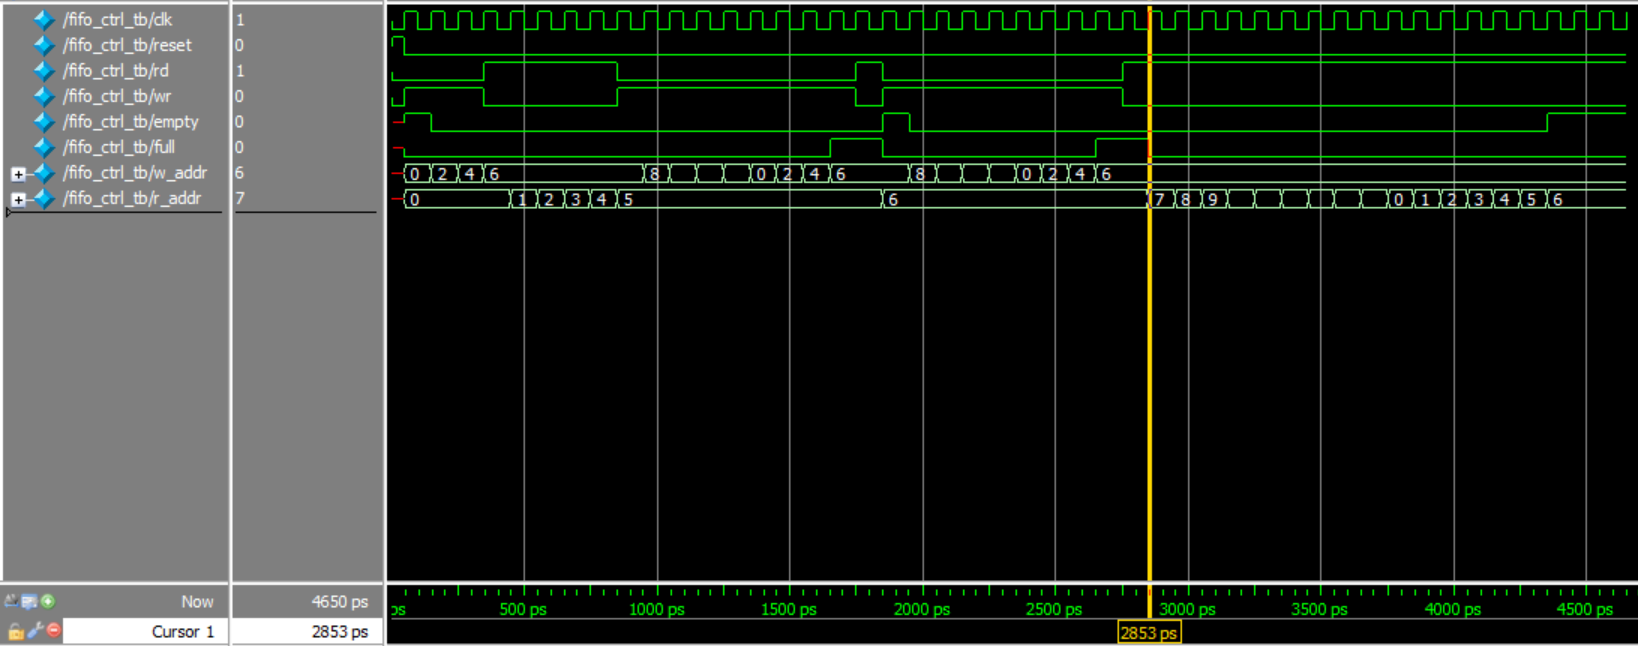
\includegraphics[scale=0.5]{Images/fifo ctrl simulation.png}
            \end{center}

            Fifo Simulation:
            \begin{center}
                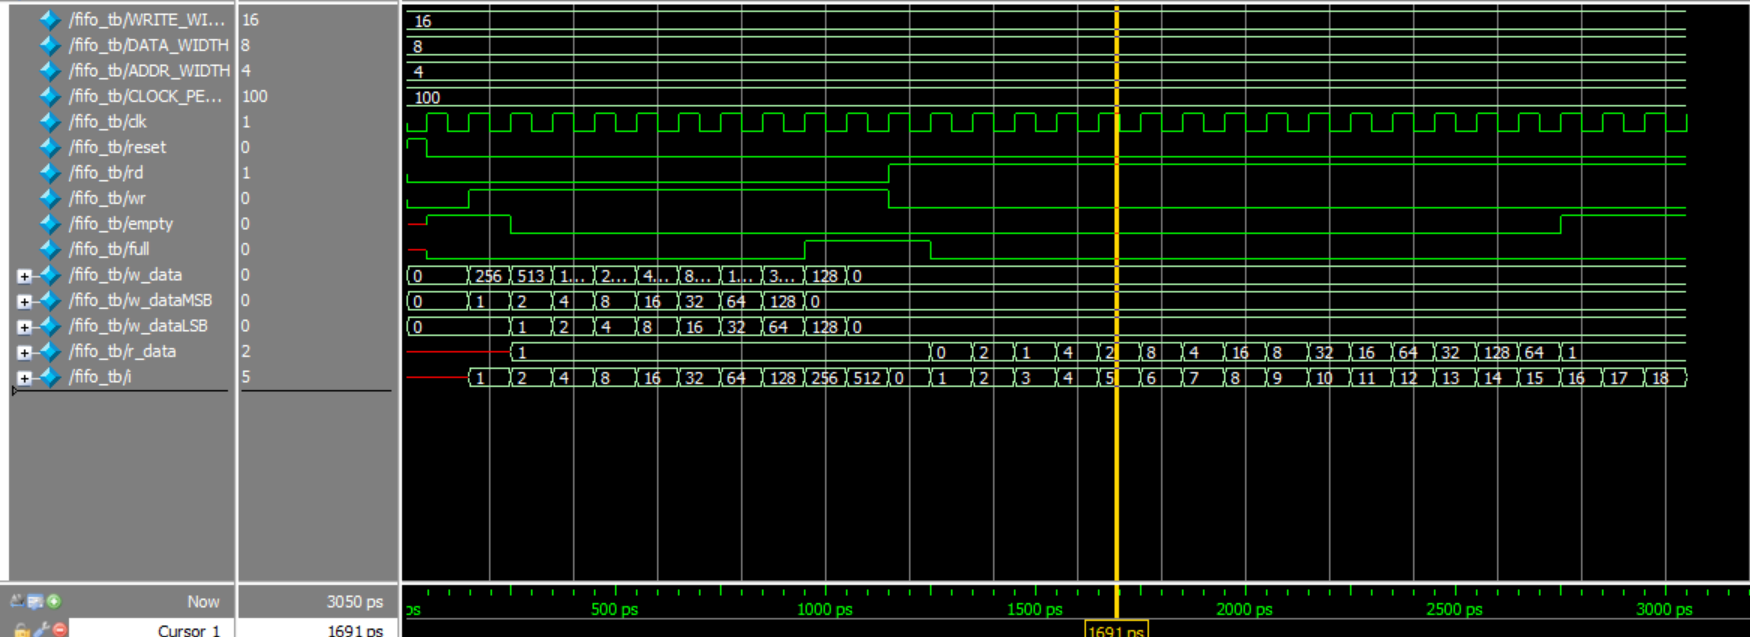
\includegraphics[scale=0.5]{Images/fifo simulation.png}
            \end{center}
        \end{subquestion}

    % Question 2
    \section{}
        \begin{explanation}
            \begin{center}
                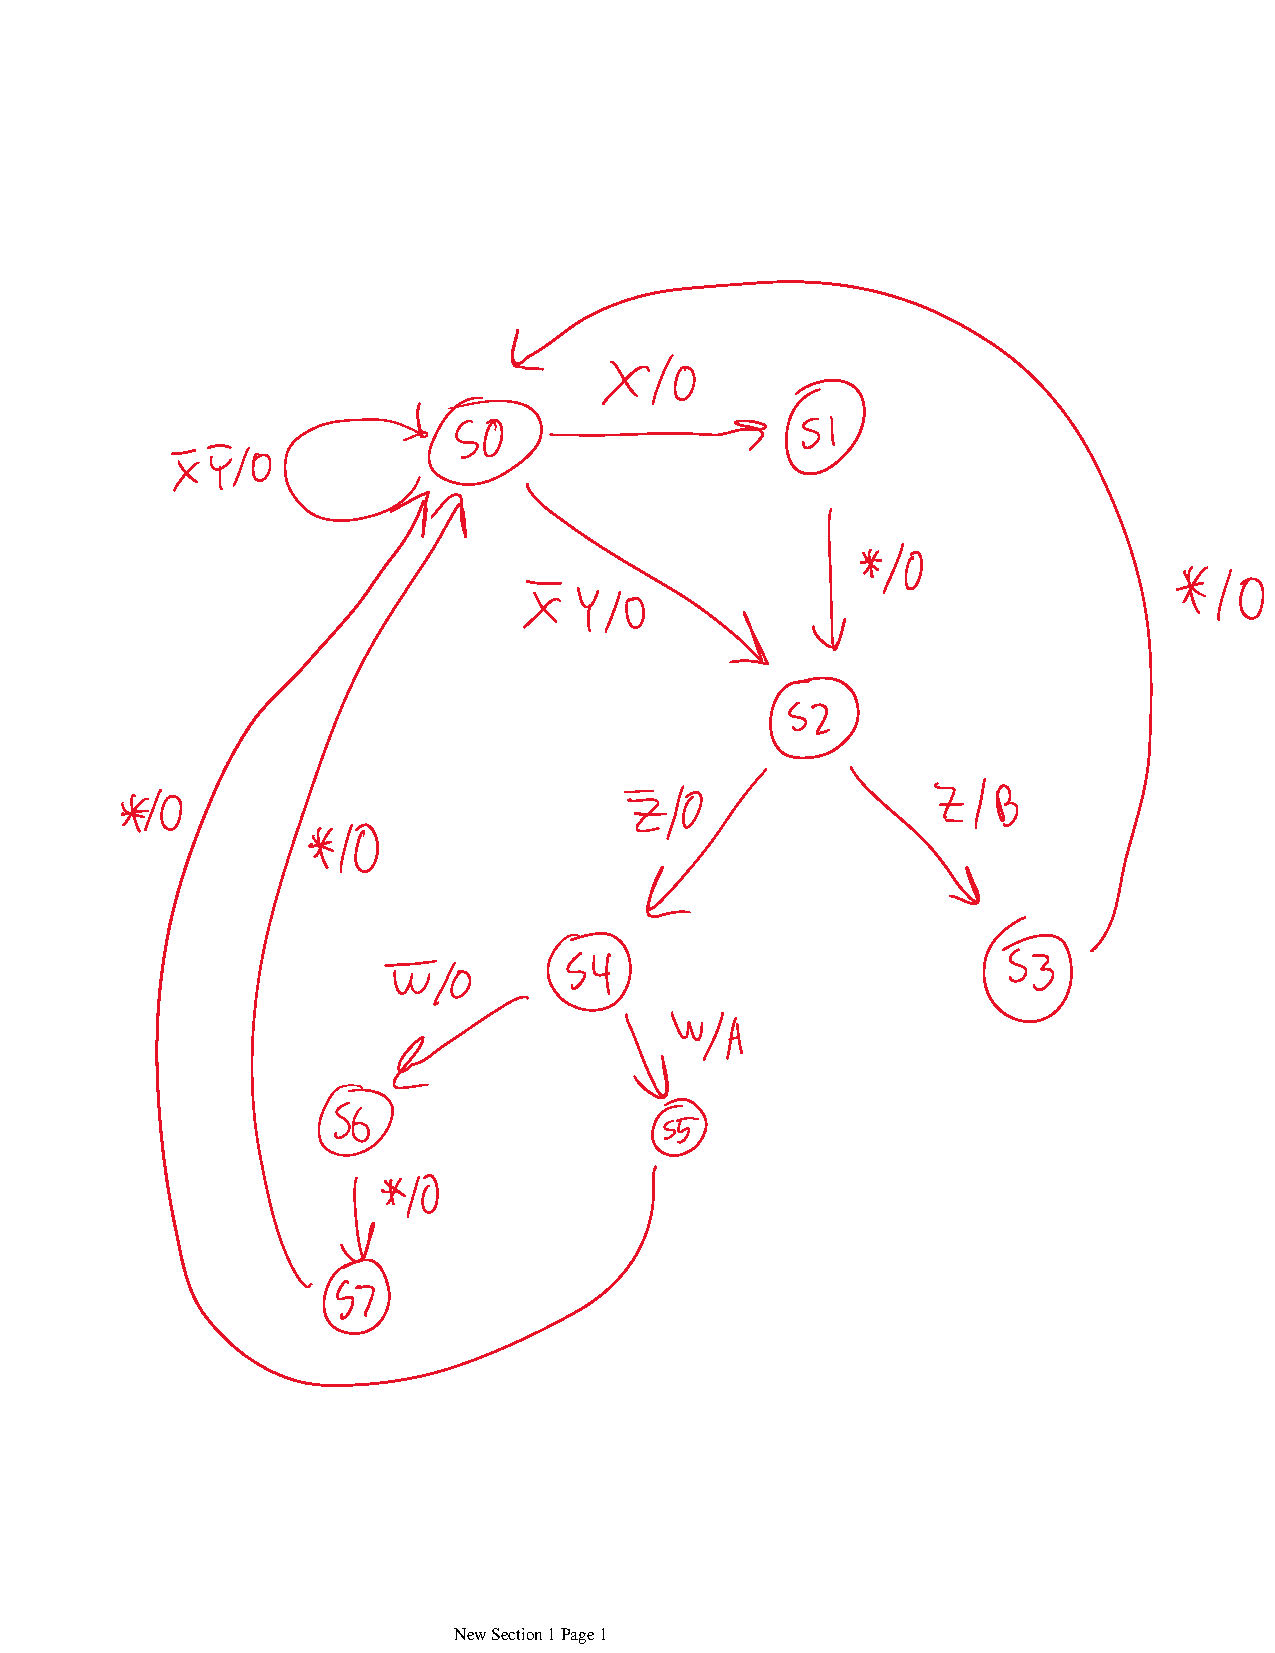
\includegraphics[scale=0.7]{Images/problem 2 fsm diagram.pdf}
            \end{center}
        \end{explanation}
        
    % Question 3
    \section{}
        \begin{subquestion}{Describe/explain the difference in timing between the Moore and Mealy outputs. How do the ASM blocks help indicate the timings?}
            The difference in timing is due to mealy being asynchronous while moore is syrchnous. Moore output is dependent on the state of the machine which is synced with the clock. Therefore when the clock updates the state, the output will be triggered at the same instant. However with Mealy machines, the output is also dependent on the input to the system, which can occur at anytime. Considering the state of the machine is idle between clock cycles, a proper input can trigger an output do to a combination of state and input. Thefore, the output for a Mealy machine can change at any point in time regardless of clock. The ASM blocks indicate timing because the Mealy outputs come after the state block which may contain Moore outputs. So, the distinction of which type of output it is, is made clear in an ASM chart. 
            
        \end{subquestion}

        \begin{subquestion}{In your opinion, how does tracing an ASM chart compare to tracing an FSM diagram.}
            We think ASM charts are cleaner to look at. We also think that FSM diagrams are easier to translate into verilog. However with an chart, it is easier to see the computations that are happening / why the hardware is designed the way it is. 
        \end{subquestion}

    \section{Experience Report}
        We found this homework to be somewhat simple and short. Problem 1 was definitely the most confusing and took the most time. 
        \begin{description}
            \item[Question 1:] 2 hours
            \item[Question 2:] 20 minutes
            \item[Question 3:] 45 minutes
        \end{description}        
\end{document}
